% kapitel4.tex
\chapter{Implementation}
\label{chapter:realisierung}
Now, that a basic abstract model is designed a implementation in Cinco can be made. Like shown in figure \ref{fig:ModelLayers} a separation of the layers will result in four different \gls{mgl} files. This leads to four different models which have to be combined with the feature already introduced called prime references. For each of them an example will be appended to clarify the proper handling and to understand the meaning of each modeling step.

\section{MGL}
\label{sec:mgl}
Even though the style definitions using \gls{msl} are very minimal in this case the focus is set on the model \gls{mgl} files.
First of all the sensor layer should be described as the rest of the model is based on this step.
\subsection{Sensor}
The one and only node without any child nodes is called metric (\cref{lst:nodeMetric}) and describes a metric like introduced in \cref{chapter:grundlagen}. 
\begin{listing}[H]
	\begin{minted}{\mgllexer}
		@style(sensorMetric, "${label}")
		@icon("src/main/resources/icons/file-export-solid.16.png")
		node Metric {
			outgoingEdges (ContainedBy)
			attr EString as label := ""
		}
	\end{minted}
	\caption{Implementation of Metric Node}
	\label{lst:nodeMetric}
\end{listing}
As shown a metric has a label describing its function like power or humidity. It has to represent the names of the metrics which are exported through the Prometheus interface. A metric can have multiple connections to different sensors but not more than one connection to a sensor.

Senors combine these metrics (line 4, figure \ref{fig:CodeSensorDevice}) into a group of exportable data. This step is done and needed for modeling real world sensor devices. This devices can be reused everywhere in the project since it is an abstract and not a concrete instance of the device holding configuration or being used. 

Attributes like a name and a specific icon  can also be edited. The names for the sensors are used to keep them apart. For a better \gls{ui} experience it is possible to select a symbol from a preselected set of icons to show up in the node. This makes it easier to get a faster coordination in bigger networks. This feature gets enabled by the $SensorIconValueProvider$ class linked with the $@possibleValuesProvider$ annotation (listing \ref{lst:classSensorIconValueProvider}).
\begin{listing}[H]
	\begin{minted}{\mgllexer}
	@style(sensorDevice, "${name}")
	@palette("DeviceDefinition")
	node DeviceDefinition {
		incomingEdges (ContainedBy)
		attr EString as name := ""
		@possibleValuesProvider("dev.schoki.metricarchitect.provider .SensorIconValueProvider")
		attr EString as icon
	}	
	\end{minted}
	\caption{Impl. of DeviceDefinition Node}
	\label{fig:CodeSensorDevice}
\end{listing}
For a faster access to the tooling some presets are implemented setting a predefined icon.
\subsection{Floor}
The modeled sensor using the previous \gls{mgl} definition can now be instantiated and configured. This can be achieved using the node $Device$. Via prime reference a link to a $DeviceDefinition$ is created (lines 4-6, \ref{fig:CodeSensorDeviceInstance}). Since it is not a specific real world device a symbolic name and a \gls{url} has to be set. The name is only used for better readability and the \gls{url} is essential. It will be generated into the Prometheus configuration for the deployment. Every node of this type corresponds to a device observed by Prometheus. 

To create a improved overview and handling a simple grouping is also implemented. This can be done by using the $Filter$ edges from the $Device$ to a $DeviceGroup$. For example it is possible to combine all power sockets or lights to one node to make them better accessible in the later steps. 

\begin{listing}[H]
	\begin{minted}{\mgllexer}
	@style(sensorInFloorModel, "${name}")
	@icon('src/main/resources/icons/bolt-solid.16.png')
	node Device {
		@pvLabel (name)
		@pvFileExtension ("sensor")
		prime SensorModel::DeviceDefinition as sensor
		outgoingEdges (GroupBy)
		attr EString as name := "DeviceName"
		attr EString as url := "localhost:8080"
	}	
	\end{minted}
	\caption{Implementation of Device Node}
	\label{fig:CodeSensorDeviceInstance}
\end{listing}

The generators for the needed configurations will follow later (see \cref{sec:impl_generator}). For a better understanding where the devices are in the real world it is possible to use the $FloorImage$ node. It has only one variable which can be set to the path of an image inside the project relative to the root. Preferably a floor plan is used. With this creating device instances without forgetting which node matches with which real world device can be easily achieved.

\subsection{Grafana}

Using the previous devices and device groups it is not possible to model the Grafana configuration. Instead, it start by creating a new node via prime reference which is than embedded into a $GraphQueryForGroup$ or for non groups $GraphQueryForDevice$ node. Both wield the same information but it is necessary to distinguish between them because the generators act differently while processing these nodes. Since this node only works as a connection to the floor \gls{mgl} it does not contain more information. 

\begin{listing}[H]
	\begin{minted}{\mgllexer}
		@style(graphQueryForGroup, "${deviceGroup.name}")
		@icon('src/main/resources/icons/chart-line-solid.16.png')
		node GraphQueryForGroup {
			@pvLabel (name)
			@pvFileExtension ("floor")
			prime FloorModel::DeviceGroup as deviceGroup
			outgoingEdges (GraphQueryToPanel)
		}
	\end{minted}
\end{listing}

Due to this layer covering the Grafana configuration \gls{promql} queries are an essential part of it. The outgoing edge $GraphQueryToPanel$ covers a rich set of possible queries but not the overall features. It is the part of the model which describes the derived \gls{promql} query the most. Like already mentioned in subsection \ref{subsec:promql} there are different parameters to set. It is necessary to keep up to the right syntax, because the values for the variables are unchecked strings. The fields $timespan$, $timeresolution$ and $offset$ (line 6-8, listing \ref{lst:GraphQueryToPanel}) has to follow the roles for duration notation (page \pageref{lst:promql_vector}, figure \ref{lst:promql_vector}). All connected devices either connect via device groups or can directly have many different metrics. Since it does not make sense to show not compatible metrics in the same graph, like power and humidity, a value provider filters all common metrics of the devices. 

\begin{listing}[H]
	\begin{minted}{\mgllexer}
@style(simpleArrow)
edge GraphQueryToPanel {
	@possibleValuesProvider("dev.schoki.metricarchitect.provider .FilterValueProvider")
	attr EString as filter
	attr Aggregation as function := "none"
	attr EString as offset
	attr EString as timespan
	attr EString as timeresolution
}
	\end{minted}
	\caption{Implementation of the Edge connecting GraphQueryByGroup/GraphQueryByDevice to a Panel symbolizing a PromQL Query}
	\label{lst:GraphQueryToPanel}
\end{listing}

The $FilterValueProvider$ class (page \pageref{lst:classFilterValueProvider}, listing \ref{lst:classFilterValueProvider}) has to take into consideration that there are $GraphQueryByGroup$ and $GraphQueryByGroup$. This is done by a simple type checking in runtime with the java $instanceof$ keyword. Using this way a drop down menu will only allow valid metrics to be used.

Lastly an aggregation operator has to be selected. The default is $none$. This is not a function implemented by \gls{promql} but it is used as a keyword in this project for doing nothing, meaning there will not be a function around the generated query. The original \gls{promql} has many different functions and as already said, for this project only some of them are implemented. 

\begin{center}
	none | sum | min | max | avg | group | stddev | stdvar | count | count\_values | bottomk | topk  | quantile
\end{center}

It can be easily expanded but for a simple proof of concept the set is sufficient. These edges can than be merged to a $Panel$ node. At this state it does not have specific attributes. Yet, it can technically have all needed properties which can be used for setting up a Grafana panel. This could be width and height, position in x and y coordinates, graph style and so on.

With the non specific edge $PanelToDashboard$ a connection to the last node in this \gls{mgl} file can be established. The final node is the $Dashboard$ node. It is not very interesting but it has a name which is used by Grafana as the shown identifier. Additionally a unique id has to be set to ensure the correct functionality of Grafana. This is done by using the $@postCreate$ annotation (line 3, listing \ref{lst:nodeDashboard}) and a proper class for it. The class $DashboardPostCreateSetUniqueId$ creates a random string which will be set as $internal\_id$. This value is nothing the developer has to take care of and plays only an important role for the generator.

\begin{listing}[!ht]
	\begin{minted}{\mgllexer}
	@style(dashboard, "${name}")
	@icon('src/main/resources/icons/list-alt-regular.16.png')
	@postCreate('dev.schoki.metricarchitect.hooks.grafanamodel .DashboardPostCreateSetUniqueId')
	node Dashboard {
		incomingEdges (PanelToDashboard)
		attr EString as name := ""
		final unique attr EString as internal_id := " " 
	}
	\end{minted}
	\caption{Implementation of Dashboard Node}
	\label{lst:nodeDashboard}
\end{listing}
\subsection{Project}
The Project layer was added to have a better overview. It can contain different information which can be possibly needed for better management. Extensions like adding options for the Docker deployment or specific settings for Grafana and Prometheus could be added here in future work. Furthermore it is used as an entry point for the generators. 

The one and only node in this layer is the $GrafanaModel$ node which has a prime reference to a whole Grafana layer model file. It is possible to add multiple nodes.

Like already mentioned, this layer is the beginning for the generation process. A generator is appended with a $@generatable$ ( line 3, \cref{lst:modelProjectModel}) annotation. The class $ProjectGenerator$ therefor does all necessary steps. 

\begin{listing}[!ht]
	\begin{minted}{\mgllexer}
	@style("model/General.style")
	@primeviewer
	@generatable("dev.schoki.metricarchitect.codegen.ProjectGenerator","/src-gen/")
	graphModel ProjectModel {
		...
	}
	\end{minted}
	\caption{Implementation of ProjectModel Graph Model}
	\label{lst:modelProjectModel}
\end{listing}

\section{Generators}
\label{sec:impl_generator}

Generating the needed files for deployment is done by $ProjectGenerator$ class. It calls generators for the three different products to be used. First configuration files for Prometheus are getting created by $PrometheusConfigGenerator$ using the associated template file. All defined and used sensors are collected and the necessary entries are created in the configuration (\cref{lst:xtend_prom}).

\begin{listing}
	\begin{minted}{xtend}
		«FOR s : devices.stream.filter(Utils.distinctByKey([ x | x.name])).collect(Collectors.toList())»
		- job_name: '«s.name»'
		static_configs:
		- targets: ['«s.url»']
		«ENDFOR»
	\end{minted}
	\caption{Part of Prometheus Configuration Template for Setting Sensors}
	\label{lst:xtend_prom}
\end{listing} 

Grafana therefor requires more files. The files worth mentioning are the dashboard definitions. They are created by traversing trough the tree of nodes while gathering all queries defined in each $GraphQueryToPanel$ edge. This leads to multiple panels with multiple queries in each dashboard. The responsible class is $GrafanaConfigGenerator$.

Finally the $docker-compose.yml$ file is created by $DockerComposeGenerator$. In this file nothing is altered dynamically. In this generator parameters do not have an effect in generation. However, to be still able to develop a more complex deployment in further iterations of this project a template was created.

\section{Cinco Product}

In the Cinco Product generated by Cinco using the models described above~\ref{sec:mgl} domain experts can realize recapture their sensor networks. From now on we call this explicit generated \gls{ide} product MetricArchitect. 

\begin{figure}
	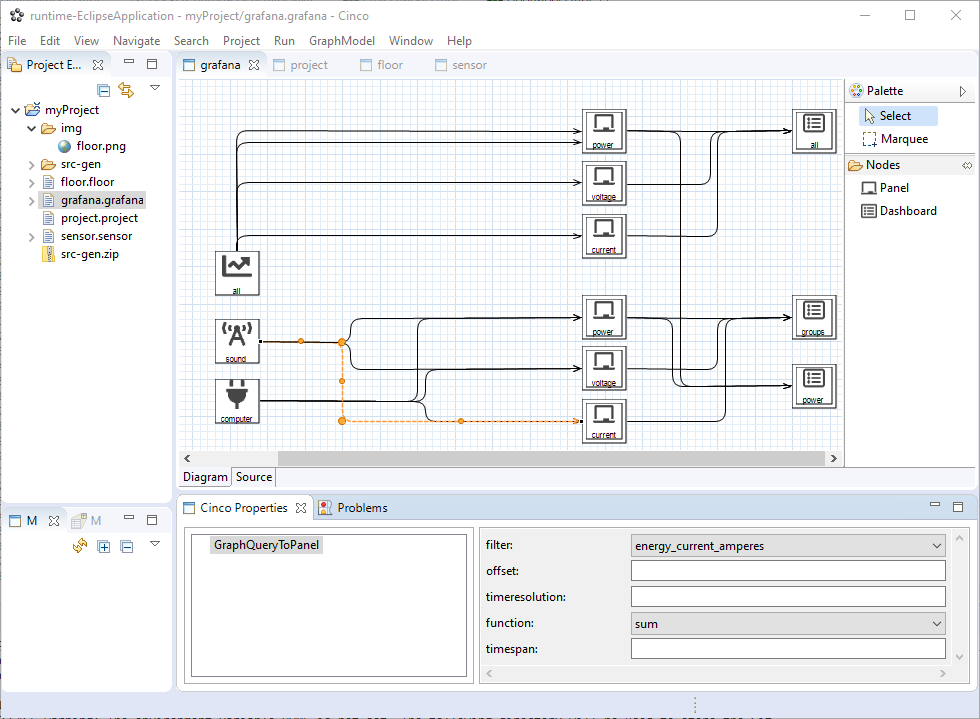
\includegraphics[width=\textwidth]{assets/images/editor}
	\caption{Screenshot of generated Cinco \gls{ide}}
	\label{fig:editor}
\end{figure}

On the left hand side the project structure is visible. For each layer one file was created. The $img$ folder has the images used in the modeling process. In the center of the screen the modeling area can be found. If elements are selected in the lower section of the window properties can be set.

To understand the example better the notation will be introduced.

\subsection{Sensor Layer}

\subsubsection{Metric}
\noindent\begin{minipage}{0.15\textwidth}%
	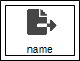
\includegraphics[width=\linewidth]{assets/images/metric}
\end{minipage}%
\hfill%
\begin{minipage}{0.8\textwidth}
	For creating metrics this node type is used. The text \say{name} is a visual placeholder for any string.
\end{minipage}


\subsubsection{Device Definition}
\noindent\begin{minipage}{0.15\textwidth}%
	
\includegraphics[width=\linewidth]{assets/images/sensor7}
\end{minipage}%
\hfill%
\begin{minipage}{0.8\textwidth}
	This is the default sensor node. The string \say{name} is a placeholder. This can be the sensor model. Since different sensor type exist some specializations are possible to use. These specialized nodes have a preset icon. In the default node this icon is changeable.
\end{minipage}

\begin{figure}[!ht]
	\centering
	\subfloat{
		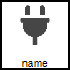
\includegraphics[width=0.08\linewidth]{assets/images/sensor1}
	}\qquad
	\subfloat{
		
\includegraphics[width=0.08\linewidth]{assets/images/sensor2}
	}\qquad
	\subfloat{
		
\includegraphics[width=0.08\linewidth]{assets/images/sensor3}
	}\qquad
	\subfloat{
		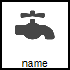
\includegraphics[width=0.08\linewidth]{assets/images/sensor4}
	}\qquad
	\subfloat{
		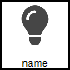
\includegraphics[width=0.08\linewidth]{assets/images/sensor5}
	}\qquad
	\subfloat{
		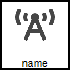
\includegraphics[width=0.08\linewidth]{assets/images/sensor6}
	}\qquad
	\subfloat{
		
\includegraphics[width=0.08\linewidth]{assets/images/sensor7}
	}\qquad
\end{figure}

\noindent
The versions of the node can be used to give hints what the technical device is measuring.

\subsection{Floor Layer}

\subsubsection{Device}
\noindent\begin{minipage}{0.15\textwidth}% adapt widths of minipages to your needs
	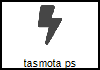
\includegraphics[width=\linewidth]{assets/images/sensor}
\end{minipage}%
\hfill%
\begin{minipage}{0.8\textwidth}
	Concrete Devices are mapped by these nodes. This node can be created by using prime references. Therefor $DeviceDefinition$ nodes has to be pulled into the modeling screen. The icon is inherited from the referenced node.
\end{minipage}

\subsubsection{Device Group}
\noindent\begin{minipage}{0.15\textwidth}%
	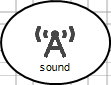
\includegraphics[width=\linewidth]{assets/images/group}
\end{minipage}%
\hfill%
\begin{minipage}{0.8\textwidth}
	This node can be used to sum up a number of Device nodes in one superordinate Node. This act like a group. In contrast to the other node it is round to be better distinguishable in the floor layer.
\end{minipage}

\subsubsection{Floor Image}
\noindent\begin{minipage}{0.15\textwidth}%

\includegraphics[width=\linewidth]{assets/images/dummy2}
\end{minipage}%
\hfill%
\begin{minipage}{0.8\textwidth}
A background can be set in the floor layer to create a better overview about the positioning of the devices. Since this node is optional a dummy image showing a diagonal bar is set a default.
\end{minipage}


\subsection{Grafana Layer}

\subsubsection{Graph Query For Device}
\noindent\begin{minipage}{0.15\textwidth}%
	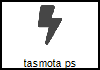
\includegraphics[width=\linewidth]{assets/images/sensor}
\end{minipage}%
\hfill%
\begin{minipage}{0.8\textwidth}
	In the Grafana Layer this node can be used to reference a already defined device from the floor layer by prime reference. The icon is inherited from the referenced node.
\end{minipage}

\subsubsection{Graph Query For Group}
\noindent\begin{minipage}{0.15\textwidth}%
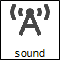
\includegraphics[width=\linewidth]{assets/images/group2}
\end{minipage}%
\hfill%
\begin{minipage}{0.8\textwidth}
In the Grafana Layer this node can be used to reference a already defined device group from the floor layer by prime reference. Since technically it does not make a difference if this is a single device or a group it has the same appearance as the $GraphQueryForDevice$ node. The icon is inherited from the referenced node.
\end{minipage}


\subsubsection{Panel}
\noindent\begin{minipage}{0.15\textwidth}%
	
\includegraphics[width=\linewidth]{assets/images/panel}
\end{minipage}%
\hfill%
\begin{minipage}{0.8\textwidth}
	The two different graph query nodes can be connected into panels. The edges to the panels have the important data to create the queries in the generation process. This node corresponds to panels in Grafana. 
\end{minipage}

\subsubsection{Dashboard}
\noindent\begin{minipage}{0.15\textwidth}%
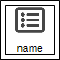
\includegraphics[width=\linewidth]{assets/images/dashboard}
\end{minipage}%
\hfill%
\begin{minipage}{0.8\textwidth}
	Dashboards consists of multiple panels. Since this is a generated solution it is possible to share panels between different dashboards. 
\end{minipage}



\subsection{Project Layer}

\subsubsection{Grafana Model}
\noindent\begin{minipage}{0.15\textwidth}%
	
\includegraphics[width=\linewidth]{assets/images/project}
\end{minipage}%
\hfill%
\begin{minipage}{0.8\textwidth}
	Since this layer has meta information for the project and acts as an entrypoint for the generation every Grafana model has to be included here through prime references.
\end{minipage}

\section{Example}

The first thing to do is creating a new $MetricArchitectTool$ Project. In general a project can look like in \cref{fig:editor}.  

To wrap everything up and show how the different layers work with each other an example project will be set up. Multiple smart power sockets were used for this. In this case the Gosund SP1 (\cref{fig:gosund_sp1}) with a flashed firmware. 

The open source project Tasmota \cite{tasmotawebsite} which is licensed under \gls{gpl3} is an alternative firmware for a huge amount of different \gls{iot} devices such as lights, switches, curtains or power sockets like the ones used in this example.
With the version 8.5.1 which was released on 2nd October 2020 Tasmota gets optional support for Prometheus exports. 

\begin{figure}[!ht]
	\centering
	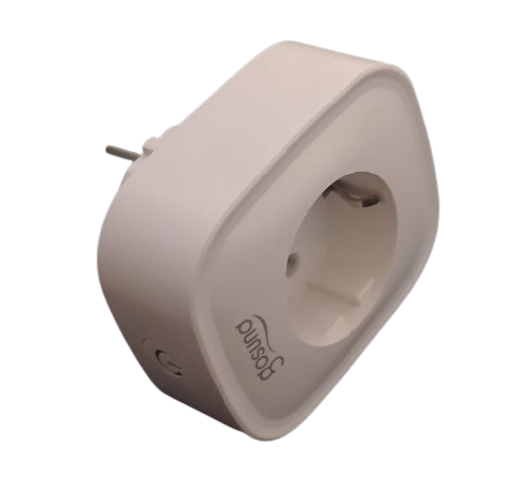
\includegraphics[width=4cm]{assets/images/gosund.png}
	\caption{Gosund SP1 Smart Power Socket}
	\label{fig:gosund_sp1}
\end{figure}

Connecting to the correct \gls{url} under $/metrics$ will then return a well formatted Prometheus export (\cref{lst:exGosundExport}).

\begin{listing}[!ht]
	\begin{minted}{text}
		# TYPE energy_voltage_volts gauge
		energy_voltage_volts 239
		# TYPE energy_current_amperes gauge
		energy_current_amperes 0.218
		# TYPE energy_power_active_watts gauge
		energy_power_active_watts 36
	\end{minted}
	\caption{Part of the Export of Gosund SP1 with Tasmota Firmware. Unimportant metrics are not shown.}
	\label{lst:exGosundExport}
\end{listing}

These three metrics are the one which should be modeled in the Cinco product. The following metrics has to be created using the metric node type. 

\begin{itemize}
	\item $energy\_voltage\_volts$
	\item $energy\_current\_amperes$
	\item $energy\_power\_active\_watts$ 
\end{itemize}

Additionally a new device definition is needed. In this case it will be named $tasmota\ ps$. Each of the created metrics needs than to be connected to the device definition (\cref{fig:modeled_sensor_layer}).

\begin{figure}[!ht]
	\centering
	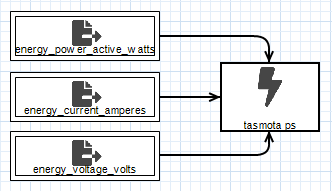
\includegraphics[width=.7\linewidth]{assets/images/sensorLayer}
	\caption{Modeled Sensor in the Sensor Layer}
	\label{fig:modeled_sensor_layer}
\end{figure}

Based on this model the real world scenario will be created. It is not only important to know that a sensor exist, but also to have some metadata of it. The position and ip are the needed data here. Across two rooms (\cref{fig:modeled_floor_layer}) four of the smart power sockets were placed. Two of them in the office and two more in the living room. Each of Bob's and Alice's computer is now monitored by such a smart socket. Additionally a \gls{hifi} audio system and the corresponding sub woofer in the living room are going to be observed. To make the handling easier a grouping is introduced. A group named $sound$ wields $hifi$ and $subwoofer$, group $computer$ has $bob$ and $alice$. The last group $all$ has each device connected to it. The floor plan was created in Sweet Home 3D is also open source and free to use~\footnote{\url{http://www.sweethome3d.com/}}. 

\begin{figure}[!ht]
	\centering
	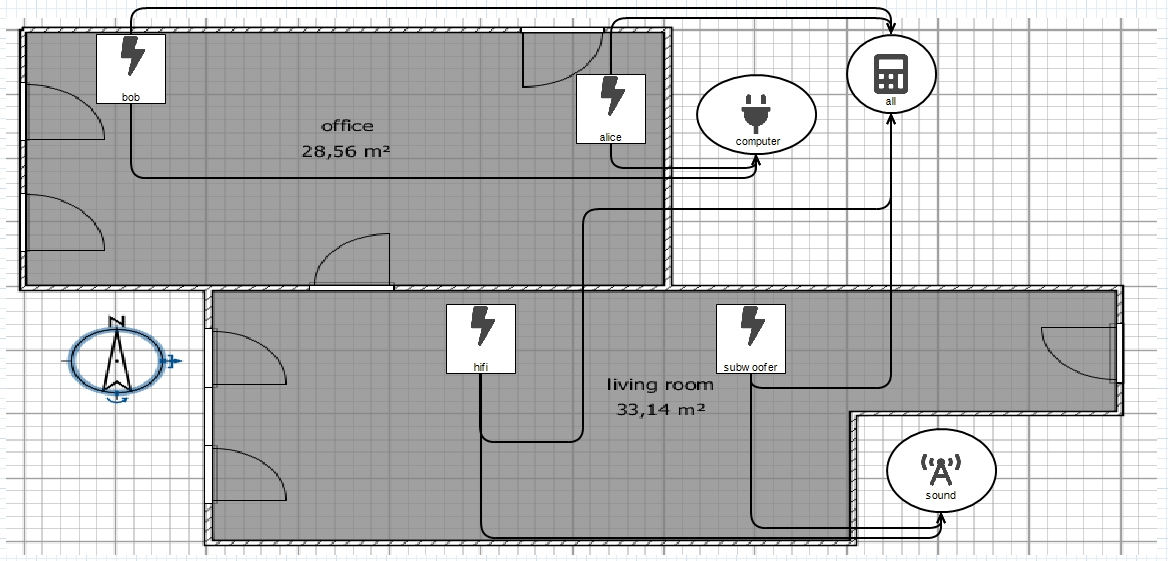
\includegraphics[width=\linewidth]{assets/images/floorLayer}
	\caption{Modeled Floor in the Floor Layer}
	\label{fig:modeled_floor_layer}
\end{figure}

After completing the translation of the upper scenario into the model the next step is to form the \gls{promql} queries and define which query goes in which panel. Afterwards the panels has to be grouped into dashboards. The most work has to be done configuring the edges from the device nodes to the panels.

From the floor layer the groups are included via prime references into the Grafana layer as seen on the left hand side in figure \ref{fig:modelGrafanaLayer}. From the $all$ node following connections are done:

\begin{itemize}
	\item Sum of $energy\_power\_active\_watts$ to power panel
	\item All $energy\_power\_active\_watts$ to power panel
	\item All $energy\_current\_amperes$ to current panel
 	\item All $energy\_voltage\_volts$ to voltage panel
\end{itemize}

This results in every power consumption shown in the panel view. As an addition the sum of all these values will be drawn. The panels for current and voltage do not contain any accumulated values but only the raw measured metrics. All three panels are then merged in the dashboard called $all$.

On the other side the group $sound$, combines the $hifi$ and $subwoofer$ device. The edges filters for each power, current and voltage. For a better overview for power and current the sum and for voltage the average will be calculated. 

The $groups$ dashboard has the panels which show the values of the group $sound$ and $computer$. Both power panels are both displayed in the power dashboard.

\begin{figure}[!ht]
	\centering 
	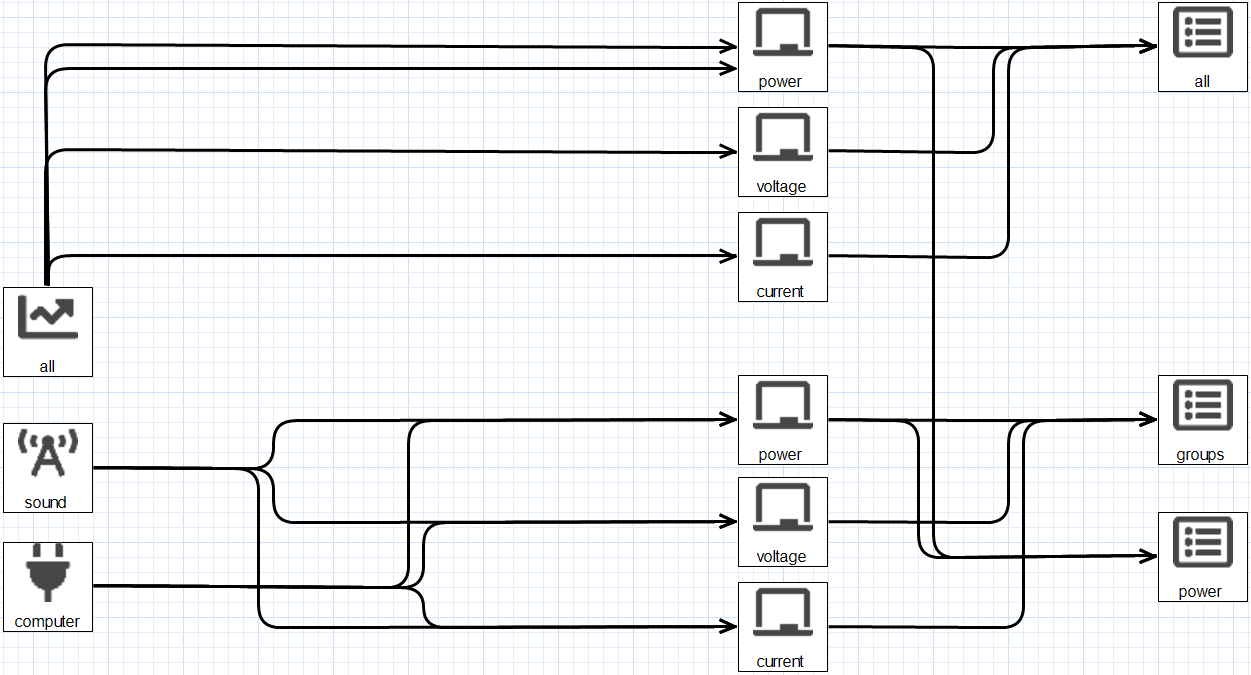
\includegraphics[width=\linewidth]{assets/images/grafanaLayer}
	\caption{Modeled Grafana in the Grafana Layer}
	\label{fig:modelGrafanaLayer}
\end{figure}

The last layer for the project level is very minimal and has only one node with the name $Main$ (\cref{fig:modeled_project_layer}).

\begin{figure}[!ht]
	\centering
	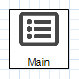
\includegraphics{assets/images/projectLayer}
	\caption{Modeled Project in the Project Layer}
	\label{fig:modeled_project_layer}
\end{figure}

After generating this project the  deployment is simple. Different configuration files are getting generated. A full tree view can be found in \cref{lst:treeview}. For Prometheus the $prometheus.yml$ file is created. It has all information inside which are needed to listen to the sensors and grab their values for further processing. Unlike Prometheus, Grafana needs more information. A file for the data source definition having all needed parameters for a valid connection between Prometheus and Grafana and a file $dashboards\_config.yml$. The later contains meta information, like the organizations name, but also describes where Grafana can find the generated dashboard definitions. These definitions are also the last of the three components being generated. Panels used across multiple dashboards can not be created once and shared but have to be generated multiple times and saved in each dashboard definition file.

\begin{listing}[!ht]
	\setlength{\DTbaselineskip}{20pt}
	\dirtree{%
		.1 src-gen\DTcomment{generated code}.
		.2 dashboards.\DTcomment{all generated dashboards}.
		.3 B3FGrzJVje.json.
		.3 Hx7CdOX0sH.json.
		.3 jjtD4JnHQa.json.
		.2 dashboards\_config.yml\DTcomment{Grafana configuration}.
		.2 docker-compose.yml.
		.2 grafana\_prometheus\_connection.yml\DTcomment{data source settings for Grafana}.
		.2 prometheus.yml\DTcomment{Prometheus configuration}.
	}
	\caption{Tree View of Generated Files}
	\label{lst:treeview}
\end{listing}

For this the template functions of Xtend was heavily used. Skeleton configuration files were extended using the template function feature. To collect all needed data to finalize the configuration files simple tree traversing through the different layers of nodes was used. Additionally some helper functions were written for formatting and composing the gathered information. 

The generated Prometheus Configuration has all placed sensors devices from the model. Every sensor having its own \glossary{ip} address and name is mentioned in the file. \cref{lst:generated_prometheus_yaml} shows four entries from the sensor devices placed in the office and living room with their defined names.

\begin{listing}[!ht]
	\begin{minted}{yaml}
		static_configs:
		- targets: ['192.168.0.233:80']
		- job_name: 'alice'
		static_configs:
		- targets: ['192.168.0.230:80']
		- job_name: 'hifi'
		static_configs:
		- targets: ['192.168.0.231:80']
		- job_name: 'subwoofer'
		static_configs:
		- targets: ['192.168.0.232:80']
	\end{minted}
	\caption{Part of Generated Prometheus Configuration File}
	\label{lst:generated_prometheus_yaml}
\end{listing}

The dashboard definition files are long and cannot be shown here as they contain 300 lines. Therefor important part will be shown. The queries have more parameters then the expression but in this work only the expression is getting generated. \cref{lst:dashboard_expr} shows how the queries are stored in the dashboard definition. The $refId$ is auto generated since it is only needed for Grafana.

\begin{listing}[!ht]
	\begin{minted}{json}
		{
			"expr": "sum(energy_power_active_watts{job=~\"bob|alice|hifi|subwoofer\"})",
			"interval": "",
			"legendFormat": "",
			"refId": "A" 
		},
	\end{minted}
	\caption{Part of a Dashboard Definition Holding Prometheus Query}
	\label{lst:dashboard_expr}
\end{listing}

A data source for Grafana has to be defined. Grafana need the right setting and connection information for using Prometheus. Since Grafana and Prometheus are deployed by Docker the necessary information are already know. \cref{lst:generated_data_source} shows the generated data source configuration without comments. It has descriptive data like a name for the connection or if it is the default database to use. As the Prometheus deployment is called $prometheus$ is the $docker\text{-}compose.yml$ the $url$ parameter can be set to \url{http://prometheus:9090}. The Docker internal domain name resolution service allows it.

\begin{listing}[!ht]
	\begin{minted}{yaml}
        apiVersion: 1
        
        datasources:
          - name: Prometheus
            type: prometheus
            access: proxy
            orgId: 1
            uid: prometheus
            url: http://prometheus:9090
            isDefault: true
            jsonData:
              graphiteVersion: '1.1'
              tlsAuth: false
              tlsAuthWithCACert: false
            version: 1
            editable: false
	\end{minted}
	\caption{Generated Grafana Data Source for Prometheus}
	\label{lst:generated_data_source}
\end{listing}

To make testing and deployment easier a $docker\text{-}compose.yml$ was created. It utilizes Docker and the Docker Compose~\cite{poulton2019docker} feature.  This allows a very fast startup and test of the generated project. The content of the generated file is shown in \cref{lst:generated_docker_compose}. Line 3 and 14 are both pods which should be deployed. The first one is responsible for Grafana. Publishing the port but more important mounting all configuration files from the model. The deployments set up for Prometheus looks similar. For the purpose of simplicity two volumes are being created. This is the place where Grafana and Prometheus can store their data.

\begin{listing}[!ht]
	\begin{minted}{yaml}
version: '3'
services:
  grafana:
    ports:
      - "127.0.0.1:3000:3000"
    volumes:
      - data-grafana:/var/lib/grafana
      - ./grafana_prometheus_connection.yml:/etc/grafana/ provisioning/datasources/grafana_prometheus_connection.yml
      - ./dashboards_config.yml:/etc/grafana/ provisioning/dashboards/dashboards_config.yml
      - ./dashboards:/var/lib/grafana/dashboards/general
    links:
      - prometheus
    image: "grafana/grafana"
  prometheus:
    ports:
      - "127.0.0.1:9090:9090"
    volumes:
      - ./prometheus.yml:/etc/prometheus/prometheus.yml
      - data-prometheus:/prometheus
    image: "prom/prometheus"
volumes:
  data-prometheus:
    driver: local
  data-grafana:
    driver: local
	\end{minted}
	\caption{Generated docker-compose.yml}
	\label{lst:generated_docker_compose}
\end{listing}

\subsection{Deployment}

As the generated file create a ready to deploy configuration a example start up is visible in \cref{fig:deployment}. Both services are started in parallel. In the terminal only the Grafana log is visible because it has a bit slower start up. Also visible are the environment variables getting  overwritten by the settings done in the $docker\text{-}compose.yml$ file.

%\begin{listing}
%	\begin{minted}{text}
%Starting src-gen_prometheus_1 ... done
%Starting src-gen_grafana_1    ... done
%Attaching to src-gen_prometheus_1, src-gen_grafana_1
%...
%prometheus_1  | level=info ts=2021-03-09T23:51:23.628Z caller=main.go:802 msg="TSDB started"
%prometheus_1  | level=info ts=2021-03-09T23:51:23.628Z caller=main.go:928 msg="Loading configuration file" filename=/etc/prometheus/prometheus.yml
%prometheus_1  | level=info ts=2021-03-09T23:51:23.629Z caller=main.go:959 msg="Completed loading of configuration file" filename=/etc/prometheus/prometheus.yml totalDuration=651.023µs remote_storage=1.563µs web_handler=305ns query_engine=704ns scrape=196.415µs scrape_sd=88.901µs notify=24.5µs notify_sd=13.811µs rules=1.493µs
%prometheus_1  | level=info ts=2021-03-09T23:51:23.629Z caller=main.go:751 msg="Server is ready to receive web requests."
%...
%grafana_1     | t=2021-03-09T23:51:24+0000 lvl=info msg="Config overridden from Environment variable" logger=settings var="GF_PATHS_DATA=/var/lib/grafana"
%grafana_1     | t=2021-03-09T23:51:24+0000 lvl=info msg="Config overridden from Environment variable" logger=settings var="GF_PATHS_LOGS=/var/log/grafana"
%grafana_1     | t=2021-03-09T23:51:24+0000 lvl=info msg="Config overridden from Environment variable" logger=settings var="GF_PATHS_PLUGINS=/var/lib/grafana/plugins"
%grafana_1     | t=2021-03-09T23:51:24+0000 lvl=info msg="Config overridden from Environment variable" logger=settings var="GF_PATHS_PROVISIONING=/etc/grafana/provisioning"
%...
%grafana_1     | t=2021-03-09T23:51:24+0000 lvl=info msg="HTTP Server Listen" logger=http.server address=[::]:3000 protocol=http subUrl= socket=
%	\end{minted}
%\end{listing}

\begin{figure}[!ht]
	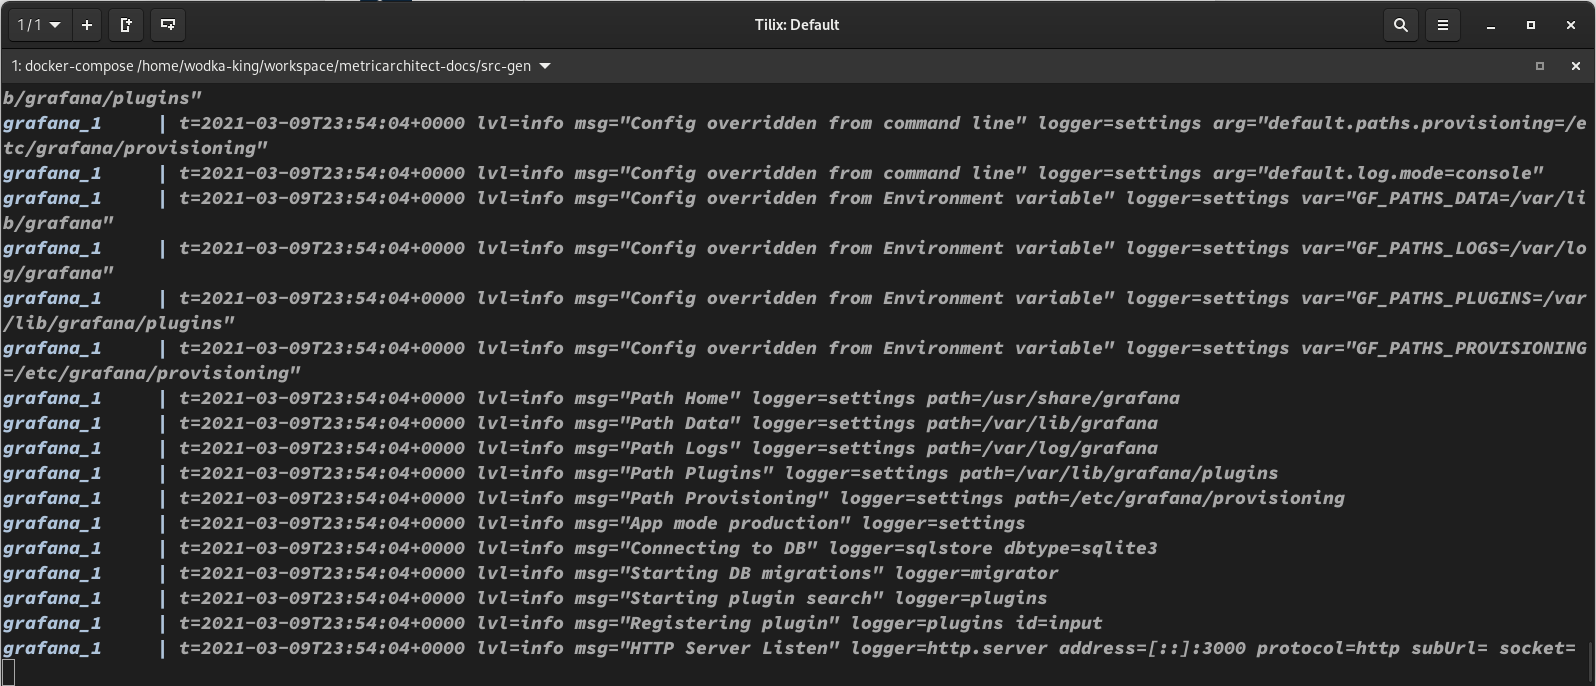
\includegraphics[width=\linewidth]{assets/images/terminal}
	\caption{Deployment with Docker Compose}
	\label{fig:deployment}
\end{figure}

Since everything started without problems the Prometheus and Grafana \gls{ui} can be tested. First of all the accessible sensor devices by Prometheus can be listed. \cref{fig:prometheus} visualizes all sensors. How long a scrap took and when the last scrap was. The state of all devices is up signaling a working connection. 

\begin{figure}[!ht]
	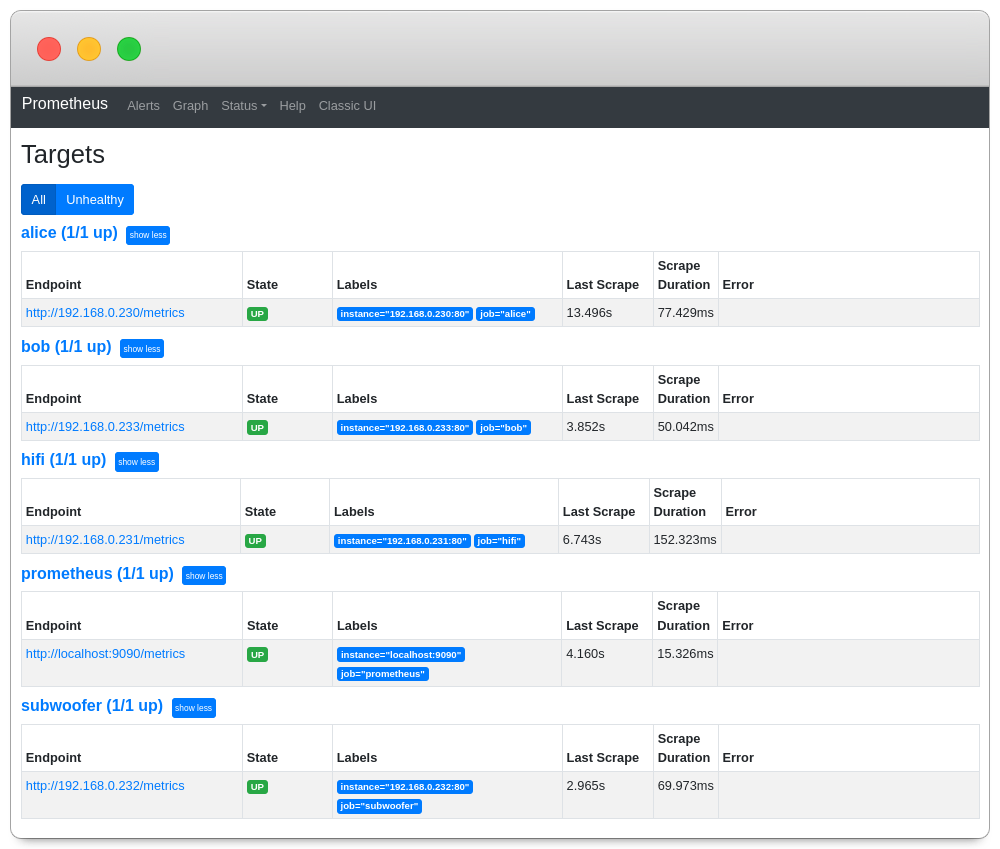
\includegraphics[width=\linewidth]{assets/images/prometheus}
	\caption{Sensor Device Overview in Prometheus}
	\label{fig:prometheus}
\end{figure}


Taking a look on the $all$ dashboard the 3 modeled panels can be found (\cref{fig:grafana}). The panel $power$, $voltage$ and $current$ show the raw information for each sensor device. Additionally a sum of the power consumption is visible in the $power$ panel. Since there is no opportunity to define the panels in size right now all panels have the same size.  


\begin{figure}[!ht]
	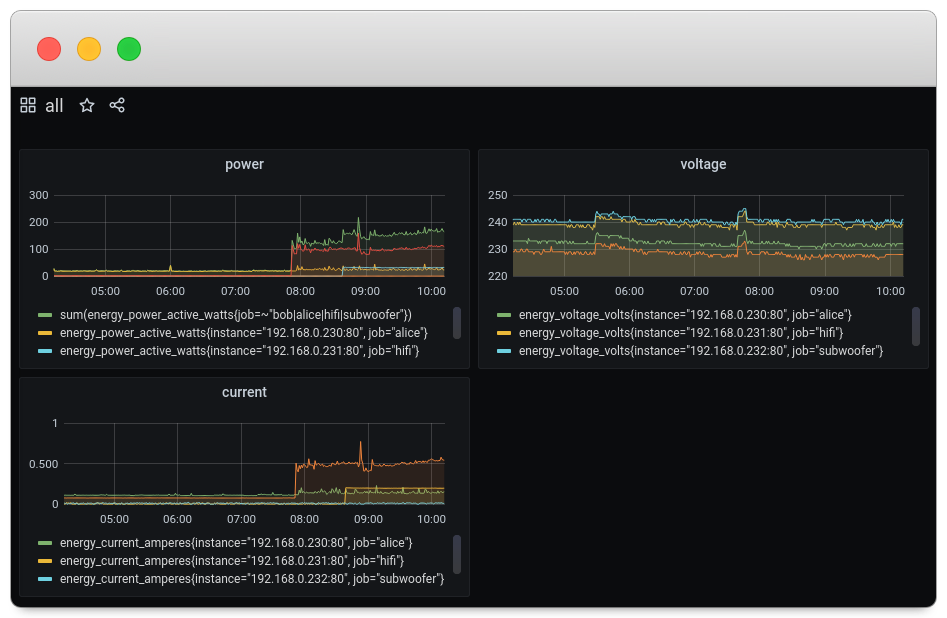
\includegraphics[width=\linewidth]{assets/images/dashboard_all}
	\caption{Example View in Generated Grafana}
	\label{fig:grafana}
\end{figure}